\documentclass{beamer} % "Beamer" is a word used in Germany to mean video projector. 
\usepackage{lmodern}
\usetheme{Luebeck} % Search online for beamer themes to find your favorite or use the Berkeley theme as in this file.
\usepackage[utf8]{inputenc}

\usepackage{color} % It may be necessary to set PCTeX or whatever program you are using to output a .pdf instead of a .dvi file in order to see color on your screen.
\usepackage{graphicx} % This package is needed if you wish to include external image files.
\usepackage[absolute,overlay]{textpos}
\usepackage{tikz}
\usetikzlibrary{calc} 
\usepackage{eurosym}



\xdefinecolor{redx}{rgb}{1,0,0}
\xdefinecolor{greenx}{rgb}{0,.7,0}
\xdefinecolor{bluex}{rgb}{0,0,.8}
\xdefinecolor{purplex}{rgb}{.7,0,.7}
\xdefinecolor{orangex}{rgb}{.9,.5,0}

\newcommand{\rgrey}[1]{{\color{greyx!40}#1}}
\xdefinecolor{greyx}{rgb}{0,0,0}

\newcommand{\rred}[1]{{\color{redx!100}#1}}
\newcommand{\ggreen}[1]{{\color{greenx!100}#1}}
\newcommand{\bblue}[1]{{\color{bluex!100}#1}}
\newcommand{\ppurple}[1]{{\color{purplex!100}#1}}
\newcommand{\oorange}[1]{{\color{orangex!100}#1}}
\renewcommand{\vec}{\mathbf}


\setbeamertemplate{headline}{}
\addtobeamertemplate{block begin}{\pgfsetfillopacity{0.88}}{\pgfsetfillopacity{1}}
 \addtobeamertemplate{block alerted begin}{\pgfsetfillopacity{0.9}}{\pgfsetfillopacity{1}}
 \addtobeamertemplate{block example begin}{\pgfsetfillopacity{0.92}}{\pgfsetfillopacity{1}}

\title{Overview of Lattice based Cryptography}
\author[Léo Ducas, CWI, Amsterdam, The Netherlands]{\Large Léo Ducas} 
\institute{CWI, Amsterdam, The Netherlands \\

\includegraphics[height = 1.8cm]{img/CWI.png}
}
\date{Spring School on Lattice-Based Cryptography \\
Oxford, March 2017} 

\newcommand{\Z}{\ensuremath {\mathbb Z}}
\DeclareMathOperator{\vol}{vol}
\DeclareMathOperator{\poly}{poly}

\AtBeginSection[]{%
  \begin{frame}<beamer>
    \frametitle{Outline}
    \tableofcontents[sectionstyle=show/shaded,subsectionstyle=hide/show/hide]
  \end{frame} 
}

\begin{document} 

\usebackgroundtemplate{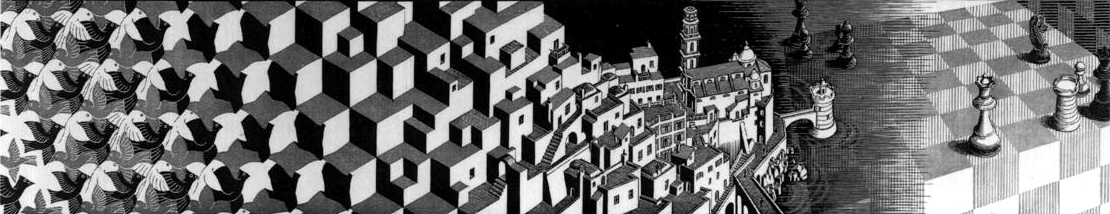
\includegraphics[width=1\paperwidth]{img/metamorphosis.png}}
\begin{frame}
\titlepage
\end{frame}
\usebackgroundtemplate{}

\begin{frame}
\frametitle{Content of the talk}
\begin{itemize}
  \item Geometric intuition behind lattice-based crypto
  \item The modern formalism (SIS-LWE)
  \item Basic construction and difficulties
\end{itemize}

  
\end{frame}

%!TEX root = main.tex

\section{The Geometric point of view}

\begin{frame}
  \frametitle{Lattices !}
\begin{figure}
\includegraphics{tikz_lattice.pdf}
\end{figure}
\begin{definition}
  A lattice $L$ is a discrete subgroup of a finite-dimensional Euclidean vector space.
\end{definition}
\end{frame}

\begin{frame}
\frametitle{Bases of a Lattice}
\includegraphics{tikz_goodbadbasis.pdf}
\\
\begin{tabular}{cccll}
 $\bblue{\vec G}$ & $ \rightarrow$ & $\rred{\vec B}$& : easy &(randomization); \\
 $\rred{\vec B}$ & $\rightarrow$ & $\bblue{\vec G}$& : hard &(LLL, BKZ, Lattice Sieve...).
\end{tabular}
\end{frame}


\begin{frame}
  \frametitle{An important invariant: the Volume}

For any two bases $\bblue{\vec G}, \rred{\vec B}$ of the same lattice $\Lambda$:
\[ \det(\bblue{\vec G}\bblue{\vec G}^t) = \det(\rred{\vec B}\rred{\vec B}^t).\]
We can therefore define:
\[ \vol(\Lambda) = \sqrt{\det(\bblue{\vec G}\bblue{\vec G}^t)}.\]
Geometrically: the volume of any {\bf fundamental domain of $\Lambda$}. \\
\pause
\begin{alertblock}{Let $\bblue{\vec G^\star}$ be the Gram-Schmidt Orthogonalization of $\bblue{\vec G}$}
$\bblue{\vec G^\star}$ is ${\bf not}$ a basis of $\Lambda$, nevertheless:
\[\vol(\Lambda) = \sqrt{\det(\bblue{\vec G^\star}\bblue{\vec G^\star}^t)} = \prod \|\bblue{\vec g_i^\star}\|.\]
\end{alertblock}
\end{frame}

\begin{frame}
  \frametitle{What is a ``Good'' basis}
Recall that, independently of the basis $\bblue{\vec G}$ it hold that:
\[\vol(\Lambda) = \prod \|\bblue{\vec g_i^\star}\|.\]

Therefore, it is somehow equivalent that
\begin{itemize}
  \item $\max_i \|\bblue{\vec g_i^\star}\|$ is small
  \item $\min_i \|\bblue{\vec g_i^\star}\|$ is large
  \item $\kappa(\bblue{\vec G}) = \min_i \|\bblue{\vec g_i^\star}\| / \max_i \|\bblue{\vec g_i^\star}\|$ is small
\end{itemize}
\pause
\begin{exampleblock}{Good basis (rule of thumb)}
\vspace{-.5cm}
  \[\kappa(\bblue{\vec G}) = \poly(d), \qquad \forall i, \|\bblue{\vec g_i^\star}\| = \poly(d) \cdot \vol(\Lambda)^{1/d}. \]
  \vspace{-.5cm}
\end{exampleblock}
\pause
\begin{alertblock}{LLL-reduced basis (rule of thumb)}
\vspace{-.5cm}
  \[\kappa(\bblue{\vec G}) \approx (1.04)^{d}, \qquad \max_i \|\bblue{\vec g_i^\star}\| \approx (1.02)^d \cdot \vol(\Lambda)^{1/d}. \]
\vspace{-.5cm}
\end{alertblock}


\end{frame}



\begin{frame}
\frametitle{Bases and Fundamental Domains}
Each basis defines a {\bf parallelepipedic tiling}.
% Les algorithmes de Babai découpent l'espace en domaines fondamentaux {\bf parallélépipédiques} selon une base donnée.
\includegraphics{tikz_goodbadtiling.pdf}
\\
{\bf Round'off Algorithm [Lenstra, Babai]}:
\begin{itemize}
  \item<2-> Given a target \ppurple{$\vec t$}
  \item<3-> Find's $\oorange{\vec v} \in L$ at the center the tile.
\end{itemize}
\end{frame}

\begin{frame}
\frametitle{Round'off Algorithm}
\begin{tabular}{ccc}
\only<1-3>{\includegraphics{tikz_ro1.pdf}}\only<4->{\includegraphics{tikz_ro4.pdf}} & \raisebox{2cm}{
$\begin{matrix}
\uncover<2->{\times {\vec B}^{-1}} \\
\longrightarrow \\
  \\
  \\
\uncover<4->{\longleftarrow} \\   
\uncover<4->{\times \vec B} \\
\end{matrix}
$}
&
\uncover<2->{\only<1-2>{\includegraphics{tikz_ro2.pdf}}\only<3->{\includegraphics{tikz_ro3.pdf}}}
\end{tabular}
\textsc{RoundOff} Algorithm [Lenstra,Babai]:
\begin{itemize}
\item<2-> Use $\vec B$ to switch to the lattice $\mathbb Z^n$ ($\times \vec B^{-1}$)
\item<3-> round each coordinate (square tiling)
\item<4-> switch back to $L$ ($\times \vec B$)
\end{itemize}
\[\uncover<2->{\oorange{\vec t'} = \vec B^{-1} \cdot \oorange{\vec t} ;} 
\quad \uncover<3->{\ppurple{\vec v'} = \lfloor \oorange{\vec t'} \rceil;}
\quad \uncover<4->{\ppurple{\vec v} = \vec B \cdot \ppurple{\vec v'}} \] 
\end{frame}


\begin{frame}
\frametitle{Nearest-Plane Algorithm}
There is a better algorithm (\textsc{NearestPlane}) based on Gram-Schmidt Orth. $\vec B^\star$ of a basis $\vec B$:

\begin{figure}
\includegraphics{tikz_goodbadNP.pdf}
\end{figure}
\begin{itemize}
  \item Worst-case distance: $\frac 1 2 \sqrt {\sum \|\vec b_i^\star\|^2}$ \hfill (Approx-CVP)
  \item Correct decoding of $\oorange{\vec t} = \ppurple{\vec v} + \vec e$ where $\vec v \in \Lambda$ if \hfill (BDD) \[\|\vec e\| \leq \min \|\vec b_i^\star\| \] 
\end{itemize}

\end{frame}

 
\begin{frame}
\frametitle{Trapdoors from Lattices ?}
With a good basis $\bblue{\vec G}$ one can solve Approx-CVP / BDD.\\
Given only a bad basis $\rred{\vec B}$, solving CVP is a {\bf hard problem}. \vspace{.4cm}\\

\includegraphics{tikz_goodbadCVP.pdf}
\vspace{.4cm}\\
Can this somehow be used as a trapdoor ?
\end{frame}


\begin{frame}
  \frametitle{Encryption from lattices (simplified)}
  Using the (second) decoding algorithm, one can recover $\vec v, \vec e$ from $\vec w = \vec v + \vec e$ when 
 \[ \|\vec e \| \leq \min \| \vec b_i^*\| \]


Fix a parameter $\eta$:
\begin{itemize}
  \item Private key: good basis $\bblue{\vec G}$ such that $\|\vec g_i^*\| \geq \eta$
  \item Public key: bad basis $\rred{\vec B}$ such that $\|\vec b_i^*\| \ll \eta$
  \item Message : $\vec m \in \Lambda = \mathcal L(\rred{\vec B}) = \mathcal L(\bblue{\vec G})$
  \item Ciphertext : $\vec c = \vec m + \vec e$, for a random error $\vec e$, $\|\vec e\| \leq \eta$
  \item Decryption : $(\vec m', \vec e) = \textsc{NearestPlane}(\vec c)$
\end{itemize}

\end{frame}




\begin{frame}
  \frametitle{Encryption from lattices}
  
Decryption : $(\vec m', \vec e) = decode(\vec c)$\\
\includegraphics{tikz_goodbadDEC.pdf}
\begin{itemize}
  \item With the good basis $\bblue{\vec G}$, $\vec m' = \vec m$
  \item With the bad basis $\rred{\vec B}$, $\vec m' \neq \vec m$ : decryption fails !
\end{itemize}

\end{frame}


\begin{frame}
\frametitle{Signatures}

{\bf Sign}
\begin{itemize}
  \item Hash the message to a random vector $\ppurple{\vec m}$.
  \item apply \textsc{NearestPlane} with a good basis $\bblue{\vec G}$: \\
    \quad find $\oorange{\vec s} \in L$ close to $\ppurple{\vec m}$ .
\end{itemize}
\vspace{.2cm}
{\bf Verify}
\begin{itemize}
  \item check that $\oorange{\vec s} \in L$ using the bad basis $\rred{\vec B}$
    \item and that $\ppurple{\vec m}$ is close to $\oorange{\vec s}$.
\end{itemize}
\vspace{.2cm}
\includegraphics{tikz_goodbadSIGN.pdf}
\end{frame}


\begin{frame}
\frametitle{A statistical attack~[NguReg06,DucNgu12]}
The difference $\vec s - \vec m$ is always inside the parallelepiped spanned by the good basis $\bblue{\vec G}$ (or its GSO $\bblue{\vec G^\star}$):
\begin{figure}
{\centering{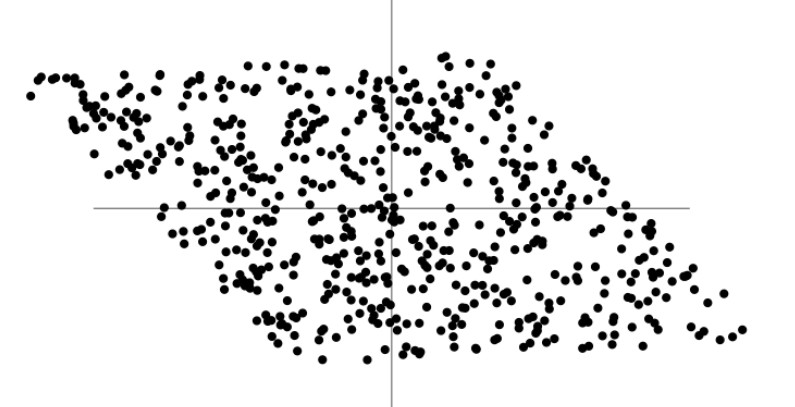
\includegraphics[width=6cm]{img/learning.jpg}}}
\end{figure}
Each signatures $(\vec s,\vec m)$ leaks a bit of information about $\bblue{\vec G}$. \\
{\bf Learning a parallepiped} from few signatures [Nguyen Regev 2006]: \\
$\quad \Rightarrow$ Total break of original GGH and NTRUSign schemes. \\
\end{frame}


\begin{frame}
\frametitle{Gaussian sampling}
Randomize the previous algorithms (Gaussian-sampling): \\
the distribution $\vec s - \vec m$ can be made {\bf independent} of $\bblue{\vec G}$
\begin{itemize}
  \item{} [Klein 2000, Gentry Peikert Vaikuthanathan 2008]: \\
  {\scriptsize Slow and memory heavy, even in the {\bf ring-setting} (NTRU, Ring-LWE)}
  \item{} [Peikert 2010] \\
  {\scriptsize Faster and less memory, but worse quality}
  \item{} [D. Prest 15] (Fast Fourier Orthogonalization) \\
  {\scriptsize Fast and good quality for certain rings}

\end{itemize}
\end{frame}

%!TEX root = main.tex

\section{The SIS-LWE Framework}

\begin{frame}
\frametitle{Construction of $q$-ary lattice (Primal / Construction A)}

Let $q$ be a prime\footnote{Not necessarly, but simpler.} integer, and $n < m$ two positives integers.

The matrix $\vec A \in \Z_q^{m \times n}$ spans the $q$-ary lattice:
\begin{align*}
\Lambda_q(\vec A) := & \,\{\vec x \in \Z^m \, | \, \exists \vec y \in \Z_q^n, \, \vec x \equiv \vec A \vec y \bmod q\}  \\
= & \,\, \vec A \cdot \Z_q^n + q \Z^m
\end{align*}
\begin{exampleblock}{Lattice parameters}
Assuming $\vec A$ is full-rank:
\begin{itemize}
  \item $\dim(\vec A) = m$
  \item $\vol(\vec A) = q^{m - n}$
\end{itemize}
\end{exampleblock}
\end{frame}

\begin{frame}
\frametitle{Construction of $q$-ary lattice (Dual / Parity-Check)}

Let $q$ be a prime\footnote{Not necessarly, but simpler.} integer, and $n < m$ two positives integers. \\
The matrix $\vec A^{\rred t} \in \Z_q^{\rred{n \times m}}$ is the parity-checks the lattice:
\begin{align*}
\Lambda_q^\bot(\vec A^{\rred t}) := & \,\{\vec x \in \Z^m \, | \vec A^{\rred t} \vec x \equiv \vec 0 \bmod q\}  \\
= & \ker (\vec x \mapsto \vec A^{\rred t} \vec x \bmod q) \phantom{\Z_q^n}
\end{align*}
\begin{exampleblock}{Lattice parameters}
Assuming $\vec A$ is full-rank:
\begin{itemize}
  \item $\dim(\vec A) = m$
  \item $\vol(\vec A) = q^{\rred n}$
\end{itemize}
\end{exampleblock}
\end{frame}


\begin{frame}
\frametitle{The Short Integer Solution Problem (SIS)}
\begin{definition}[SIS assumption]
  Given a random matrix 
  Finding a small non-zero $\vec x \in \Z_q^n$ such that $\vec A \vec x \equiv \vec 0 \bmod q$ is {\bf hard}. \\
\end{definition}
\begin{exampleblock}{Lattice formulation}
  Solving Approx-SVP in $\Lambda_q^\bot(\vec A^t)$ is {\bf hard}.
\end{exampleblock}
\pause
\end{frame}

\begin{frame}
\frametitle{Simple application of SIS}
Set $\mathcal S = \{0, 1\}^m$ and consider the function:
\[
  f_{\vec A}: \mathcal S \rightarrow \Z_q^n, \qquad \vec x \mapsto \vec A^t \vec x \bmod q
\]

\begin{exampleblock}{SIS $\Rightarrow$ Collision Resistant Hashing and One-Way Function}
  \begin{itemize}
    \item Finding collision\footnote{Collision must exist whenever $m > n \log_2 q$} is as hard as SIS \hfill {\scriptsize (take the difference)}
  \end{itemize}
  Moreover, if $m \gg n \log q$:
  \begin{itemize}
    \item $f_{\vec A}$ is highly surjective \hfill {\scriptsize (many pre-images exists)}
    \item Finding pre-images is hard.
  \end{itemize}
\end{exampleblock}
\end{frame}

\begin{frame}
\frametitle{The Learning With Error problem (LWE)}
Let $\chi$ be a distribution of small errors $\ll q$. 
\begin{definition}[Decisional LWE]
For $\vec A \gets \Z_q^{m \times n}$, $\vec s \gets \Z_q^{n}$, $\bblue{\vec e} \gets \chi^m$, \\ distinguishing $(\vec A, \vec A \vec s + \bblue{\vec e})$ from uniform is hard.
\end{definition}
\begin{definition}[Search LWE]
For $\vec A \gets \Z_q^{m \times n}$, $\vec s \gets \Z_q^{n}$, $\bblue{\vec e} \gets \chi^m$, \\ given $(\vec A, \vec A \vec s + \bblue{\vec e})$, finding $\vec s$ is hard.
\end{definition}
Both problems are easily proved equivalent.
\pause
\begin{exampleblock}{Lattice formulation}
  Solving BDD in $\Lambda_q(\vec A)$ is {\bf hard}.
\end{exampleblock}
\end{frame}

\begin{frame}
\frametitle{Simple application of LWE}
Set $\mathcal S = \{-\sigma, \dots \sigma\}^m$ and consider the function:
\[
  g_{\vec A}: \Z_q^n \times \mathcal S \rightarrow \Z_q^m, \qquad (\vec s, \bblue{\vec e}) \mapsto \vec A \vec s + \bblue{\vec e} \bmod q
\]

\begin{exampleblock}{LWE $\Rightarrow$ Secret-Key Encryption}
  Idea : Noisy one-time pad
  \begin{itemize}
    \item $Enc_{\vec s}(m\in\{0,1\} ) = (\vec a,\vec a^t \vec s + e + \lfloor \frac q 2 \rceil m)$ 
    \item $Dec_{\vec s}(\vec a, b ) = \lfloor \frac 2 q (b - \vec a^t \vec s) \rfloor \bmod 2$ 
  \end{itemize}
\end{exampleblock}
\end{frame}

\begin{frame}
\frametitle{Public Key Encryption, [Regev, 2009]}
$m \gg n \log q$.
\begin{itemize}
  \item $SK = \vec s \in \Z_q^m$
  \item $PK = (\vec A; \vec b = \vec A \vec s + \bblue{\vec e}) \in \Z_q^{(n+1) \times m}$
  \item $Enc(m) = (\bblue{\vec t^t} \cdot \vec A, \bblue{\vec t^t} \cdot \vec b + \lfloor \frac q 2 \rceil m + e)$, where $\vec t \gets \{0,1\}^{n+1}$
  \item $Dec(\vec x^t, y):$ Compute $d = y - \vec x^t \vec s = \bblue{\vec t^t} \bblue{\vec e} + e + \lfloor \frac q 2 \rceil m$, return
   $m = \lfloor \frac 2 q d \rfloor \bmod 2$
\end{itemize}
\pause
\begin{exampleblock}{Proof sketch for CPA security}
\begin{itemize}
  \item Replace PK by uniform random $(\vec A, \vec b)$
  \item Apply the left-over hash lemma on $\vec t$ over $(\mat A, \vec b)$
  \item $Enc(m)$ is staitistically close to uniform.
\end{itemize}
\end{exampleblock}
\end{frame}

\begin{frame}
\frametitle{PKE / Approx. Key-Exchange [Lindner Peikert 2011]}
Using a Systematic-Normal form, one can assume that $\bblue{\vec s} \gets \chi^n$ is small as well.
Take $m = n$.

\begin{itemize}
  \item $PK = \vec s \in \Z_q^n$
  \item $SK = (\vec A; \vec b = \vec A \bblue{\vec s} + \bblue{\vec e}) \in \Z_q^{(n+1) \times n}$
  \item $Enc(m) = (\vec A^t \bblue{\vec s'} + \bblue{\vec e'}, \vec b^t \bblue{\vec s'} + \bblue{\vec e'} + \bblue e + \lfloor \frac q 2 \rceil m)$

  \item $Dec(\vec x, y):$ Compute $d = y - \vec x^t \vec s = \bblue{\vec s^t} \bblue{\vec e'} + \bblue{\vec s'^t} \bblue{\vec e} + e + \lfloor \frac q 2 \rceil m$, return
   $m = \lfloor \frac 2 q d \rfloor \bmod 2$
\end{itemize}
\pause
\begin{exampleblock}{Proof sketch for CPA security}
\begin{itemize}
  \item Replace PK by uniform random by LWE assumptuion
  \item Replace $Enc(m)$  by uniform random by LWE assumptuion
\end{itemize}
\end{exampleblock}
Can also be made an approximate key Exchange.
\end{frame}


\begin{frame}
\frametitle{Chosen-Ciphertext Secure ?}
Is the above CCA-secure ?
\begin{alertblock}{ NO !}
\end{alertblock}
Generic Transform to CCA security in the Random Oracle Model?
\pause
\begin{exampleblock}{Yes}
Correctness needs to hold with overwhelming probability. 
\end{exampleblock}
\pause
And in the plain Model ?
\begin{exampleblock}{Yes}
But costly: requires Trapdoors (e.g [Micciancio Peikert 2012])
Open question: Cramer-Shoup for lattices ?
\end{exampleblock}



\end{frame}
%!TEX root = main.tex

\section{Encryption is easy}

\begin{frame}
\frametitle{Encryption is easy}

{\bf Idea:}
\begin{itemize}
  \item Use one short lattice vector {\hfill \scriptsize(rather than a full good basis $\bblue{\vec B}$)}
  \item This short vector is easy to hide: LWE as unique-SVP
\end{itemize}
\end{frame}

\begin{frame}
\frametitle{Public Key Encryption, [Regev 2005]}
$m \gg n \log q$.
\begin{itemize}
  \item $SK = \vec s \in \Z_q^m$
  \item $PK = (\vec A; \vec b = \vec A \vec s + \bblue{\vec e}) \in \Z_q^{(n+1) \times m}$
  \item $Enc(m) = (\bblue{\vec t^t} \cdot \vec A, \bblue{\vec t^t} \cdot \vec b + \lfloor \frac q 2 \rceil m + e)$, where $\vec t \gets \{0,1\}^{n+1}$
  \item $Dec(\vec x^t, y)$ Compute \[d = y - \vec x^t \vec s = \bblue{\vec t^t} \bblue{\vec e} + e + \lfloor \frac q 2 \rceil m\] and return
   $m = \lfloor \frac 2 q d \rfloor \bmod 2$
\end{itemize}
\pause
\begin{exampleblock}{Proof sketch for CPA security}
\begin{itemize}
  \item Replace PK by uniform random $(\vec A, \vec b)$
  \item Apply the left-over hash lemma on $\vec t$ over $(\vec A, \vec b)$
  \item $Enc(m)$ is statistically close to uniform.
\end{itemize}
\end{exampleblock}
\end{frame}

\begin{frame}
\frametitle{PKE / Approx. Key-Exchange [Lindner Peikert 2011]}
Using a Systematic-Normal form, one can assume that $\bblue{\vec s} \gets \chi^n$ is small as well.
Take $m = n$.

\begin{itemize}
  \item $PK = \vec s \in \Z_q^n$
  \item $SK = (\vec A; \vec b = \vec A \bblue{\vec s} + \bblue{\vec e}) \in \Z_q^{(n+1) \times n}$
  \item $Enc(m) = (\vec A^t \bblue{\vec s'} + \bblue{\vec e'}, \vec b^t \bblue{\vec s'} + \bblue{\vec e'} + \bblue e + \lfloor \frac q 2 \rceil m)$

  \item $Dec(\vec x, y):$ Compute \[d = y - \vec x^t \vec s = \bblue{\vec s^t} \bblue{\vec e'} + \bblue{\vec s'^t} \bblue{\vec e} + e + \lfloor \frac q 2 \rceil m\] and return
   $m = \lfloor \frac 2 q d \rfloor \bmod 2$
\end{itemize}
\pause
\begin{exampleblock}{Proof sketch for CPA security}
\begin{itemize}
  \item Replace PK by uniform random by LWE assumptuion
  \item Replace $Enc(m)$  by uniform random by LWE assumptuion
\end{itemize}
\end{exampleblock}
Can also be made an approximate key Exchange.
\end{frame}


\begin{frame}
\frametitle{Chosen-Ciphertext Secure ?}

Are the above CCA-secure ?
\begin{alertblock}{NO !}
It is Additively Homomorphic therefore can't be CCA2. \\
CCA1 attacks left as an exercise.\footnote{Toy with the error and see if Dec. fails}
\end{alertblock}

Generic Transform to CCA security in the Random Oracle Model ?
\pause
\begin{exampleblock}{Yes [Peikert 2013]}
Correctness needs to hold with overwhelming probability. 
\end{exampleblock}
\pause
And in the plain Model ?
\begin{exampleblock}{Yes}
But costly: requires Trapdoors (e.g [Micciancio Peikert 2012])
Open question: Cramer-Shoup for lattices ?
\end{exampleblock}



\end{frame}
%!TEX root = main.tex

\section{Signatures are tricky}

\begin{frame}
\frametitle{Solution 1: Hash-Then-Sign}
{\bf Sign}
\begin{itemize}
  \item Hash the message to a random vector $\ppurple{\vec m}$.
  \item apply \textsc{NearestPlane} with a good basis $\bblue{\vec G}$: \\
    \quad find $\oorange{\vec s} \in L$ close to $\ppurple{\vec m}$ .
\end{itemize}
\vspace{.2cm}
{\bf Verify}
\begin{itemize}
  \item check that $\oorange{\vec s} \in L$ using the bad basis $\rred{\vec B}$
    \item and that $\ppurple{\vec m}$ is close to $\oorange{\vec s}$.
\end{itemize}
\vspace{.2cm}
\includegraphics{tikz_goodbadSIGN.pdf}
\end{frame}


\begin{frame}
\frametitle{Constructing a {\bf pseudorandom} lattice with a good basis}
\begin{definition}[The Matrix-NTRU assumption]
  For two small matrices $\bblue{\vec F}, \bblue{\vec G} \gets \chi^{n \times n}$, set $\vec H = \vec F\vec G^{-1} \bmod q$. \\
  Distinguishing $\vec H$ from uniform is hard.
\end{definition}
\pause
\begin{alertblock}{Do not overstreched !}
  Recently discovered to be significantly weaker than LWE/RingLWE for certain regime of parameters. \hfill cf. Thursday.
\end{alertblock}
\pause

\begin{itemize}
  \item $(\bblue{\vec F}, \bblue{\vec G})$ is a good partial basis of the lattice.
  \item It can be completed into a full good basis. {\scriptsize optimal params in [D. Prest Lyubashevski 2013]}
  \item  $\vec H$ provably uniform for midly large $\bblue{\vec F}, \bblue{\vec G}$ [Stehle Steinfeld 2012]
\end{itemize}






\end{frame}

\begin{frame}
\frametitle{Constructing a {\bf random} lattice with a good basis}



\end{frame}

\end{document}


